\begin{appendices}
\chapter{Vragen enquete}
\label{appendix:enquete}

\begin{itemize}
	
	
	\item Hoe vaak neem je de trein?
	\item In welk(e) verband(en) neem je de trein?
	\item Waar haal je (realtime) informatie met betrekking tot treinen vandaan?
	\item Hoe vaak ervaar je volgende gebeurtenissen wanneer je met de trein reist, en waar zoek je in deze gevallen informatie op?
	\begin{itemize}
		\item Een probleemloze rit
		\item Vertraging
		\item Afgeschafte treinen
		\item Spoorwijzigingen
		\item Informatie in stations niet up-to-date
		\item Informatie in app niet up-to-date
	\end{itemize}
	
	\item Hoe tevreden ben je over informatiebronnen voor openbaar vervoer per trein?
	\item Rangschik deze bronnen voor informatie voor openbaar vervoer per trein naar hoe vaak je ze gebruikt, van meest naar minst gebruikt.
	\begin{itemize}
		\item Website
		\item App
		\item Affiches of digitale borden in station
		\item Loketten
		\item Omgeroepen informatie
	\end{itemize}
	
	\item Welk besturingssysteem gebruik je op je (meestgebruikte) smartphone
	\item Welke app gebruik je hoofdzakelijk?
	\item Waar gebruik je deze app?
	\item Hoe tevreden ben je over de volgende zaken wanneer je je applicatie gebruikt?
	\item Hoe tevreden ben je over het mobiele netwerk tijdens een treinreis?
	\item Heb je soms last van een zeer trage of afwezige netwerkverbinding wanneer je op de trein zit, waardoor webpagina's enorm traag of  zelfs niet laden?
	\item Heb je schrik om meer mobiele data te verbruiken dan in je gsm abonnement of prepaid-bundel zit?
	\item Als je informatie over treinen wenst en deze niet opzoekt via een applicatie, wat is hiervoor dan de reden?
	\item Hoe belangrijk vind je onderstaande zaken in een app voor openbaar vervoer per trein? Rangschik van meest naar minst interessant.
	\begin{itemize}
		\item Offline zoekopdrachten
		\item Weinig data verbruiken
		\item Snel resultaten laden
		\item Mijn privacy beschermen
		\item Weinig batterij verbruiken
	\end{itemize}
	
	\item Hoe bezorgd ben je om je privacy bij het gebruik van je applicatie?
	\item Denk je dat je applicatie je locatie of reisplannen over internet verstuurt?
	\item Zou het je storen als je applicatie je locatie of reisplannen over internet verstuurt?
	\item Zou je overschakelen van je applicatie naar een andere app, als deze andere app je locatie of reisplannen niet over internet verstuurt?
	
	\item Hoe interessant vind je deze aspecten? Snelheid, privacy, offline gebruik, aanpasbare routeplanning.
	\item Stel dat je in een app de routeplanning ook kon aanpassen. Hoe interessant zou je het vinden om ook deze parameters in te kunnen stellen?
	\begin{itemize}
		\item 	Drukke treinen mijden
		\item 	Specifieke treinen mijden
		\item 	Kortere overstappen gebruiken	
		\item 	Langere overstappen gebruiken
		\item 	Enkel langs stations met lift, roltrap, ... plannen
	\end{itemize}
	\item Rangschik de volgende aspecten van Linked Connections van meest naar minst interessant: snelheid, privacy, offline gebruik, aanpasbare routeplanning.
	\item Hoe oud ben je?
	\item Wat is je geslacht?
\end{itemize}

\chapter{Resultaten enquete}
\label{appendix:report}
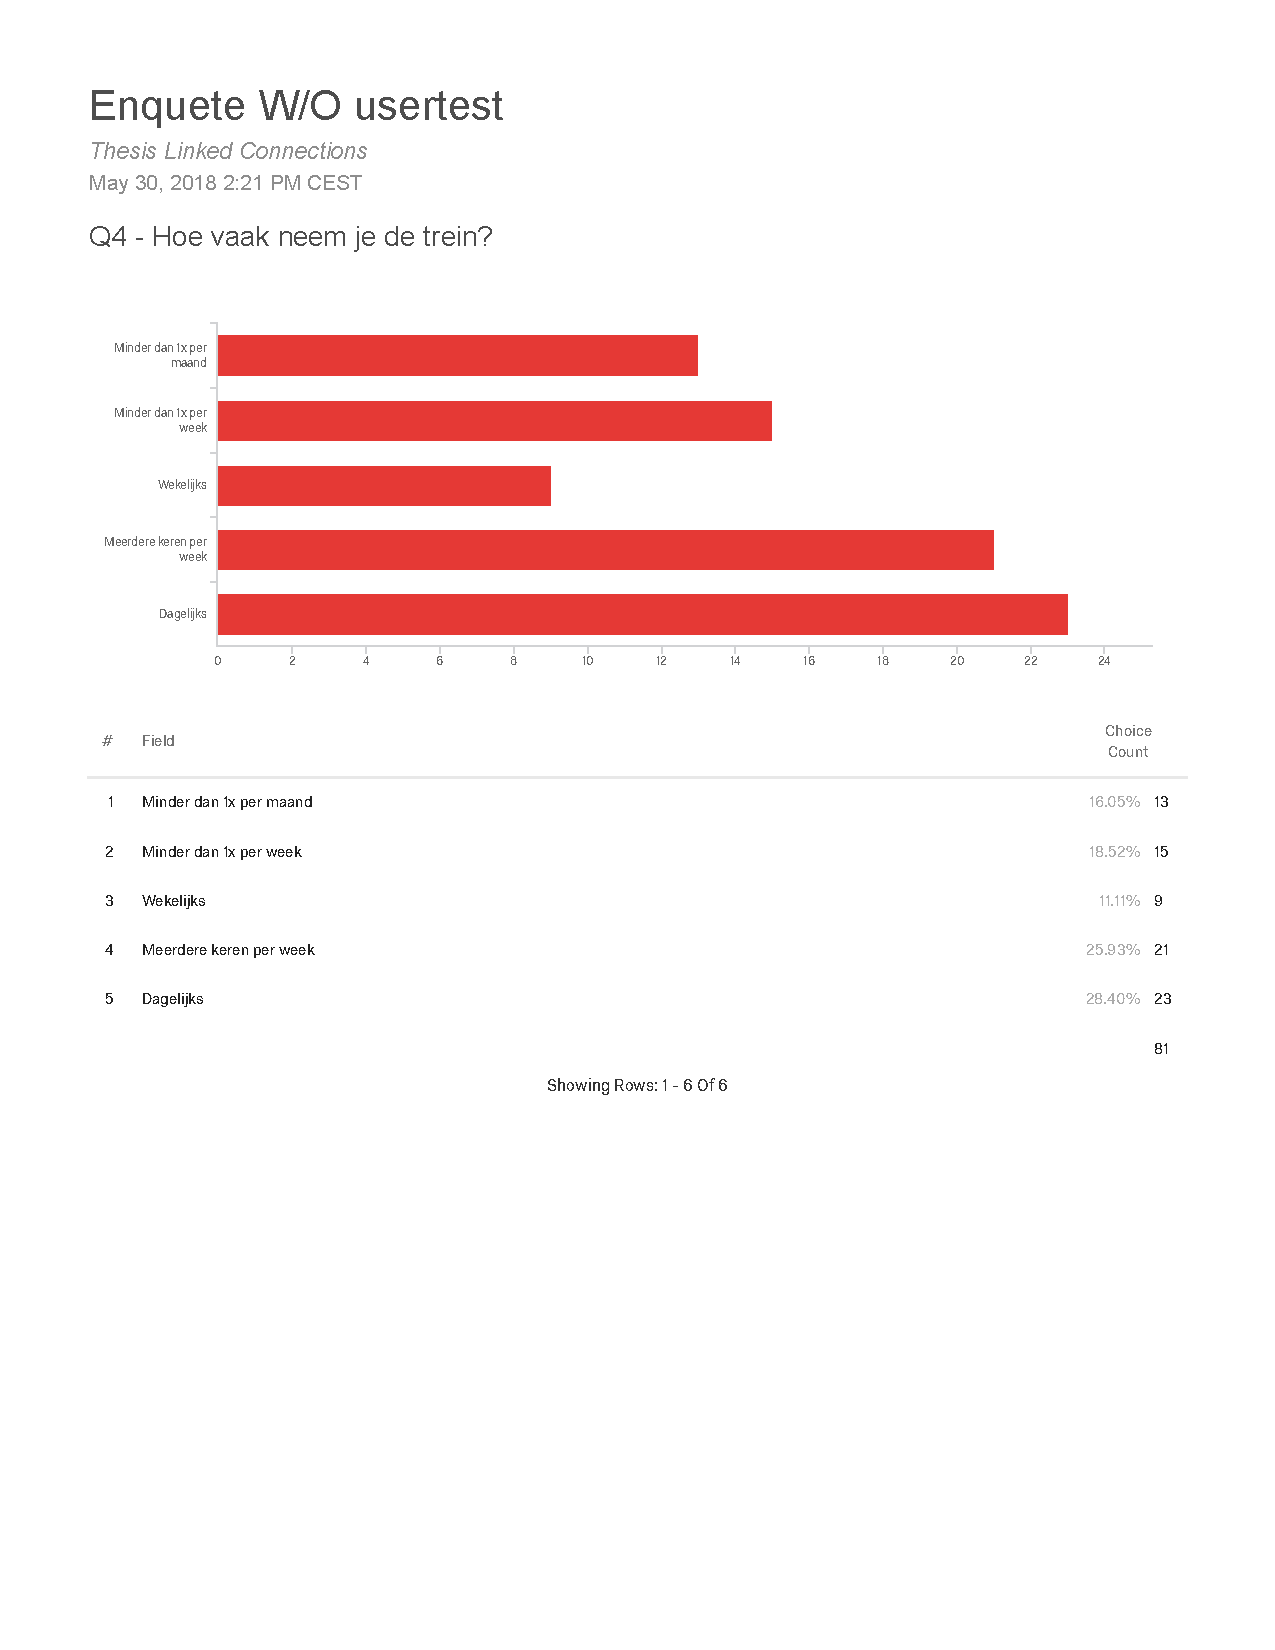
\includepdf[pages=-]{surveyreport.pdf}

\chapter{Resultaten user testing}
\label{appendix:usertesting}
\end{appendices}